\chapter{Xây dựng hệ thống Marketing Agent và phân tích kết quả thực nghiệm}\label{chap:thuc-nghiem}

Chương này trình bày toàn bộ quá trình xây dựng và thực nghiệm hệ thống:
thiết kế kiến trúc và cơ sở dữ liệu, hiện thực hóa các thành phần Agent
bằng LangGraph, thiết lập các thực nghiệm fine-tuning SFT và học tăng cường
GRPO trên dữ liệu F\&B thực tế, khung đánh giá chất lượng đa lớp, và kết
quả so sánh các phương pháp tinh chỉnh. Mọi thực nghiệm tập trung vào nền
tảng \textbf{Facebook} với dữ liệu thực tế từ các SME ngành F\&B tại Việt
Nam.

\section{Thiết kế kiến trúc hệ thống}\label{sec:kien-truc}

\subsection{Tổng quan kiến trúc}

Hệ thống được thiết kế theo mô hình \textbf{đa tác nhân} (multi-agent)
với các thành phần tách biệt rõ trách nhiệm, giao tiếp qua message queue
để đảm bảo khả năng mở rộng theo chiều ngang. Các dịch vụ cốt lõi gồm:

\begin{figure}[H]
  \centering
  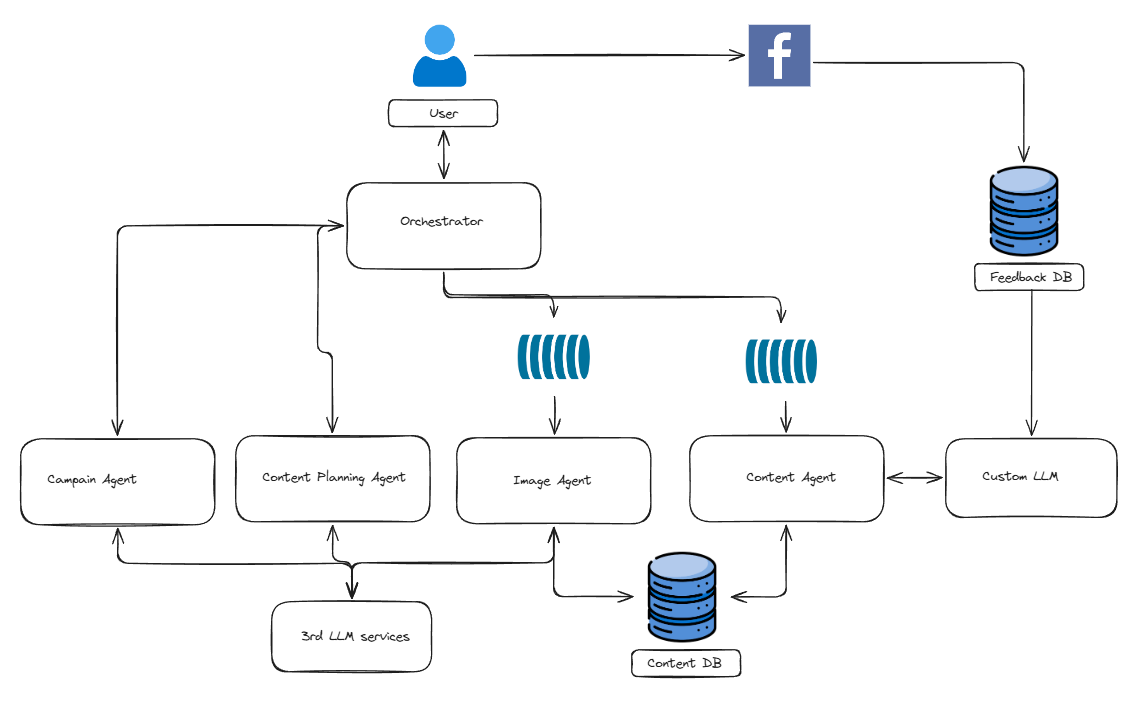
\includegraphics[width=0.95\textwidth]{images/system_architecture.png}
  \caption{Kiến trúc tổng quan hệ thống Marketing Agent}
  \label{fig:system-architecture}
\end{figure}

\begin{itemize}
  \item \textbf{Orchestrator API}: Dịch vụ FastAPI xử lý xác thực JWT,
    quản lý phiên làm việc, và là điểm vào duy nhất của người dùng. Cung
    cấp endpoint \texttt{POST /chat} nhận tin nhắn hội thoại và trả về
    phản hồi của agent cùng trạng thái chiến dịch hiện tại.
  \item \textbf{AI Agents Service}: Nhóm các Worker Celery lắng nghe ba
    hàng đợi độc lập (\texttt{content\_planning\_queue},
    \texttt{content\_queue}, \texttt{image\_queue}), mỗi hàng đợi tương
    ứng một giai đoạn trong pipeline sinh nội dung.
  \item \textbf{PostgreSQL}: Lưu trữ toàn bộ trạng thái hệ thống, lịch
    sử hội thoại, kết quả sinh nội dung và siêu dữ liệu duyệt bài.
  \item \textbf{RabbitMQ}: Message broker phân phối tác vụ nặng (gọi LLM,
    sinh ảnh) sang workers, tránh blocking luồng HTTP chính.
  \item \textbf{MinIO}: Object storage tương thích S3, lưu trữ ảnh được
    sinh ra với URL công khai cho phép nhúng trực tiếp vào bài đăng
    Facebook.
  \item \textbf{Langfuse}: Observability platform ghi lại toàn bộ lượt
    gọi LLM (prompt, response, latency, token count) phục vụ phân tích
    chi phí và debug.
  \item \textbf{LiteLLM Proxy}: Lớp trừu tượng hóa nhà cung cấp LLM,
    cho phép chuyển đổi giữa OpenAI GPT-4o, GPT-4o-mini, Claude Sonnet
    mà không thay đổi code agent.
\end{itemize}

\subsection{Cơ sở dữ liệu}\label{subsec:database}

Schema cơ sở dữ liệu được thiết kế theo ba lớp logic: nhận dạng
(identity), tri thức thương hiệu (knowledge base), và pipeline tạo nội
dung (job pipeline). Tất cả bảng dùng UUID làm khóa chính để hỗ trợ
phân tán sau này.

\subsubsection{Lớp nhận dạng và tri thức thương hiệu}

\begin{itemize}
  \item \textbf{\texttt{organizations}}: Tổ chức cấp cao nhất. Mỗi tổ
    chức sở hữu nhiều dự án và người dùng.
  \item \textbf{\texttt{projects}}: Đại diện cho một thương hiệu F\&B cụ
    thể. Lưu brand guidelines trực tiếp: \texttt{tone\_of\_voice},
    \texttt{writing\_style}, \texttt{do\_list[]},
    \texttt{dont\_list[]}. Đây là nguồn dữ liệu được nạp vào prompt của
    ContentAgent.
  \item \textbf{\texttt{users}}: Người dùng trong tổ chức, có vai trò
    \texttt{owner | admin | member}.
  \item \textbf{\texttt{products}}: Sản phẩm/món ăn của một dự án. Lưu
    thông tin marketing dạng mảng: \texttt{key\_features[]},
    \texttt{campaign\_objectives[]}, \texttt{key\_facts[]}. Mỗi lần tạo
    nội dung, agent tra cứu bảng này để lấy thông tin sản phẩm liên quan.
\end{itemize}

\subsubsection{Lớp hội thoại}

\begin{itemize}
  \item \textbf{\texttt{chat\_sessions}}: Phiên hội thoại giữa người dùng
    và CampaignAgent, gắn với một dự án. Trạng thái:
    \texttt{active | archived}.
  \item \textbf{\texttt{chat\_messages}}: Lịch sử tin nhắn trong phiên.
    Trường \texttt{role} nhận một trong bốn giá trị:
    \texttt{user | assistant | system | tool}. Trường \texttt{metadata}
    (JSONB) lưu siêu dữ liệu tùy chọn như intent phân loại hoặc ID tác
    vụ Celery liên quan.
\end{itemize}

\subsubsection{Lớp pipeline tạo nội dung}

Đây là phần cốt lõi của schema, thiết kế theo mô hình job queue phân cấp
ba tầng để cho phép retry độc lập ở mỗi bước.

\begin{itemize}
  \item \textbf{\texttt{campaign\_runs}}: Đơn vị điều phối cấp cao nhất.
    Một chiến dịch có thể sinh nhiều bài viết theo nhiều
    \emph{slot}. Trạng thái: \texttt{running | awaiting\_approval |
    completed | paused}.
  \item \textbf{\texttt{content\_planning\_jobs}}: Một slot trong chiến
    dịch, đại diện cho một yêu cầu tạo bài cụ thể. Lưu
    \texttt{slot\_index}, \texttt{attempt\_no}, \texttt{raw\_brief}
    (yêu cầu thô từ agent lập kế hoạch), \texttt{input\_title} và
    \texttt{seed\_content} (sau khi ContentPlanningAgent xử lý). Ràng
    buộc \texttt{UNIQUE(campaign\_run\_id, slot\_index, attempt\_no)}
    đảm bảo idempotency khi retry.
  \item \textbf{\texttt{content\_planning\_job\_products}}: Bảng nối
    many-to-many giữa content planning job và danh sách sản phẩm liên
    quan (một bài viết có thể quảng bá nhiều món cùng lúc).
  \item \textbf{\texttt{content\_generation\_jobs}}: Kết quả sinh nội
    dung từ ContentAgent. Lưu \texttt{headline}, \texttt{body\_markdown},
    \texttt{extra\_outputs} (JSONB — hashtags và metadata bổ sung),
    \texttt{raw\_prompt} (snapshot prompt đầy đủ để debug), và metadata
    duyệt bài: \texttt{review\_decision}, \texttt{review\_comment},
    \texttt{reviewed\_at}.
  \item \textbf{\texttt{image\_generation\_jobs}}: Kết quả sinh ảnh từ
    ImageAgent. Trường \texttt{output\_payload} (JSONB) lưu URL ảnh
    trên MinIO và các thông số sinh ảnh. Cũng có trường
    \texttt{review\_decision} để hỗ trợ luồng duyệt ảnh độc lập.
\end{itemize}

Sơ đồ quan hệ tóm tắt theo chiều từ trên xuống:
\texttt{organizations} $\to$ \texttt{projects} $\to$
\texttt{campaign\_runs} $\to$ \texttt{content\_planning\_jobs} $\to$
\texttt{content\_generation\_jobs} $\to$
\texttt{image\_generation\_jobs}.

\subsection{Luồng công việc tổng thể}

Luồng xử lý một chiến dịch đi qua bốn giai đoạn với ba hàng đợi Celery
song song:

\begin{enumerate}
  \item \textbf{Hội thoại và lập kế hoạch}: Người dùng gửi yêu cầu qua
    \texttt{POST /chat}. CampaignAgent phân loại intent; nếu là
    \texttt{REQUEST\_PLAN}, nó gọi ContentPlanningAgent để tạo
    \texttt{ExecutionPlan} (danh sách slot với brief từng bài). Kết quả
    trình bày cho người dùng phê duyệt (\texttt{awaiting\_approval}).
  \item \textbf{Phê duyệt kế hoạch}: Khi người dùng phê duyệt
    (\texttt{APPROVE\_PLAN}), CampaignAgent tạo bản ghi
    \texttt{campaign\_run} trong DB, sau đó đưa từng slot vào hàng đợi
    \texttt{content\_planning\_queue}.
  \item \textbf{Sinh nội dung}: ContentAgent worker nhận job, nạp tri
    thức thương hiệu từ \texttt{ContentRepository}, gọi LLM sinh bài
    viết và lưu vào \texttt{content\_generation\_jobs}. Song song, nếu
    kế hoạch yêu cầu ảnh, job được đưa vào \texttt{image\_queue} để
    ImageAgent xử lý.
  \item \textbf{Duyệt và đăng}: Người dùng xem kết quả, phê duyệt hoặc
    yêu cầu chỉnh sửa qua \texttt{review\_decision}. Hệ thống ghi
    nhận phản hồi vào DB làm dữ liệu cải thiện cho các chiến dịch
    sau.
\end{enumerate}

\section{Hiện thực hóa các thành phần Agent}\label{sec:hien-thuc-agent}

Tất cả agent được hiện thực trên nền tảng \textbf{LangGraph} --- thư
viện xây dựng state machine từ đồ thị có hướng trên LangChain. Mỗi
node trong đồ thị là một hàm Python nhận và trả về \texttt{AgentState}
(TypedDict); LangGraph điều phối luồng thực thi theo các điều kiện
chuyển trạng thái được định nghĩa tường minh.

\subsection{CampaignAgent --- Điều phối trung tâm}

CampaignAgent là cổng vào duy nhất của người dùng, đóng vai trò
\emph{conversational orchestrator}: hiểu ý định, lập kế hoạch, điều
phối các agent con, và duy trì bộ nhớ hội thoại liên phiên.

\textbf{State machine và chuyển trạng thái.} Agent quản lý hai chiều
trạng thái song song: \emph{ConversationState} (vòng đời hội thoại) và
\emph{ChatIntent} (ý định từng lượt). Bảng~\ref{tab:campaign-states}
tóm tắt các chuyển trạng thái hợp lệ.

\begin{table}[htbp]
  \centering
  \small
  \caption{Chuyển trạng thái hội thoại trong CampaignAgent.}
  \label{tab:campaign-states}
  \resizebox{\textwidth}{!}{%
  \begin{tabular}{llll}
    \toprule
    \textbf{Trạng thái hiện tại} & \textbf{Intent nhận được}
      & \textbf{Trạng thái tiếp theo} & \textbf{Hành động} \\
    \midrule
    \texttt{CHATTING}           & \texttt{REQUEST\_PLAN}
      & \texttt{AWAITING\_APPROVAL} & Gọi ContentPlanningAgent \\
    \texttt{AWAITING\_APPROVAL} & \texttt{APPROVE\_PLAN}
      & \texttt{DONE}               & Gọi ContentAgent + ImageAgent \\
    \texttt{AWAITING\_APPROVAL} & \texttt{REJECT\_PLAN}
      & \texttt{CHATTING}           & Xóa kế hoạch pending \\
    \texttt{AWAITING\_APPROVAL} & \texttt{CHAT}
      & \texttt{AWAITING\_APPROVAL} & Nhắc lại kế hoạch chờ \\
    \texttt{CHATTING}           & \texttt{CHAT}
      & \texttt{CHATTING}           & Trả lời tự do \\
    \bottomrule
  \end{tabular}}
\end{table}

\textbf{Kiến trúc đồ thị LangGraph.} Đồ thị có ba node chính với
điều kiện định tuyến sau node \texttt{classify}:

\begin{lstlisting}[language=Python, caption={Cấu trúc đồ thị CampaignAgent (rút gọn).}]
graph = StateGraph(CampaignState)
graph.add_node("classify", self._node_classify)
graph.add_node("plan",     self._node_plan)
graph.add_node("execute",  self._node_execute)

graph.add_edge(START, "classify")
graph.add_conditional_edges(
    "classify",
    _route,   # ham phan tich intent + conversation_state
    {"plan": "plan", "execute": "execute", END: END},
)
graph.add_edge("plan",    END)
graph.add_edge("execute", END)

checkpointer = MemorySaver()
self._app = graph.compile(checkpointer=checkpointer)
\end{lstlisting}

\textbf{Bộ nhớ liên phiên.} \texttt{MemorySaver} lưu toàn bộ
\texttt{CampaignState} (bao gồm lịch sử tin nhắn và kế hoạch đang chờ)
theo \texttt{thread\_id} là UUID phiên làm việc. Khi người dùng quay
lại cùng session, agent khôi phục đúng trạng thái từ checkpoint, không
cần gửi lại lịch sử.

\textbf{Phân loại ý định.} Node \texttt{classify} gọi LLM (GPT-4o,
$T=0{,}7$) với \emph{structured output} schema \texttt{ChatResponse}
gồm hai trường: \texttt{reply} (chuỗi phản hồi) và \texttt{intent}
(enum \texttt{ChatIntent}). Việc dùng structured output thay vì parsing
chuỗi tự do đảm bảo intent luôn hợp lệ và không cần xử lý lỗi định
dạng.

\subsection{ContentPlanningAgent --- Lập kế hoạch}

ContentPlanningAgent nhận mục tiêu chiến dịch tổng quát từ người dùng
và trả về một \texttt{ExecutionPlan} cấu trúc gồm danh sách
\texttt{Step}, mỗi step chỉ định loại tác vụ (\texttt{content\_agent}
hoặc \texttt{image\_agent}) và brief chi tiết.

Agent được hiện thực bằng \texttt{create\_agent()} của LangChain với
tập công cụ (tools) được nạp từ \texttt{TOOL\_REGISTRY} --- thiết kế
này cho phép mở rộng năng lực lập kế hoạch (ví dụ: tra cứu dữ liệu
xu hướng, kiểm tra lịch đăng bài) mà không thay đổi cấu trúc agent.
Kết quả dạng văn bản Markdown được chuyển đổi sang
\texttt{ExecutionPlan} qua hàm \texttt{build\_execution\_plan()}. Mô
hình sử dụng là GPT-5-mini ($T=1{,}0$) --- nhiệt độ cao khuyến khích
đa dạng hóa kế hoạch sáng tạo.

\subsection{ContentAgent --- Sinh nội dung}

ContentAgent là thành phần tạo ra bài viết cuối cùng. Pipeline được
thiết kế tuyến tính gồm ba node:

\[
\texttt{build\_prompt} \;\to\; \texttt{generate} \;\to\; \texttt{parse\_output} \;\to\; \text{END}
\]

\textbf{Node \texttt{build\_prompt}} nạp ngữ cảnh từ
\texttt{ContentRepository} và điền vào template
\texttt{content\_agent.md} qua \texttt{str.format()}. Template được tổ
chức thành bốn phần:

\begin{enumerate}
  \item \textbf{KNOWLEDGE BASE}: \texttt{\{product\_info\}},
    \texttt{\{brand\_info\}}, \texttt{\{key\_facts\}},
    \texttt{\{campaign\_objectives\}} --- thông tin sản phẩm và thương
    hiệu lấy từ bảng \texttt{products} và \texttt{projects}.
  \item \textbf{STYLE GUIDE}: \texttt{\{tone\_of\_voice\}},
    \texttt{\{writing\_style\}}, \texttt{\{do\_list\}},
    \texttt{\{dont\_list\}}, \texttt{\{platform\_specs\}} --- hướng
    dẫn phong cách từ brand guidelines của dự án.
  \item \textbf{GOLDEN SAMPLES}: \texttt{\{golden\_samples\}} --- các
    bài viết mẫu chất lượng cao lấy từ lịch sử \texttt{content\_generation\_jobs}
    có \texttt{review\_decision = 'approved'}, đóng vai trò few-shot
    examples.
  \item \textbf{LESSONS LEARNED}: \texttt{\{lessons\}} --- bài học
    rút ra từ các lần sinh trước, bao gồm nhận xét của người dùng khi
    từ chối bài (\texttt{review\_comment}).
\end{enumerate}

\textbf{Node \texttt{generate}} gọi LLM (GPT-4o-mini, $T=0{,}7$) với
\texttt{SystemMessage} là prompt đã điền và \texttt{HumanMessage} là
mô tả tác vụ cụ thể (tiêu đề bài, nội dung mồi). \textbf{Node
\texttt{parse\_output}} bóc tách JSON từ phản hồi thô theo schema:

\begin{lstlisting}[language=Python, caption={Output schema của ContentAgent.}]
{
  "headline": "Tieu de ngan gon duoi 15 tu",
  "body":     "Noi dung chinh cua bai viet",
  "hashtags": ["tag1", "tag2", ...]
}
\end{lstlisting}

Toàn bộ prompt thô được lưu vào trường \texttt{raw\_prompt} trong bảng
\texttt{content\_generation\_jobs} để phục vụ debug và phân tích chi phí
token qua Langfuse.

\subsection{ImageAgent --- Sinh ảnh}

ImageAgent nhận mô tả hình ảnh từ \texttt{ExecutionPlan} và sinh ảnh
qua mô hình \texttt{gpt-image-1} (DALL-E thế hệ mới). Ảnh trả về dạng
base64 PNG, được tải lên MinIO với bucket được cấu hình \emph{public-read},
và URL công khai được lưu vào trường \texttt{output\_payload} (JSONB) của
bảng \texttt{image\_generation\_jobs}.

Agent hỗ trợ cả hai chế độ: \texttt{run()} cho sinh ảnh từ đầu và
\texttt{edit()} cho chỉnh sửa ảnh đã có (người dùng cung cấp \texttt{image\_call\_id}
và mô tả thay đổi). Chế độ edit tải ảnh gốc từ MinIO về file tạm rồi
gọi \texttt{ImageModel.edit()}, hỗ trợ luồng lặp sửa ảnh mà không cần
sinh lại từ đầu.

\subsection{HTTP Service và quản lý phiên}

FastAPI service cung cấp endpoint duy nhất:

\begin{lstlisting}[language=Python, caption={Endpoint POST /chat của FastAPI service.}]
@app.post("/chat", response_model=ChatResponse)
async def chat(req: ChatRequest) -> ChatResponse:
    agent = get_or_create(req.session_id)
    output = await agent.chat(req.message)
    return ChatResponse(reply=output.reply,
                        state=output.state.value)
\end{lstlisting}

Hàm \texttt{get\_or\_create()} duy trì một dict trong bộ nhớ ánh xạ
\texttt{session\_id} tới instance \texttt{CampaignAgent}. Mỗi instance
mang \texttt{thread\_id} riêng cho \texttt{MemorySaver}, đảm bảo các
phiên làm việc độc lập về trạng thái hội thoại.

\section{Thực nghiệm fine-tuning SFT trên dữ liệu F\&B tiếng Việt}
\label{sec:fine-tuning-result}

\subsection{Thiết lập fine-tuning}

Giai đoạn này tiến hành Supervised Fine-Tuning (SFT) trên hai kích
thước tham số để đánh giá ảnh hưởng của quy mô đến hiệu quả học phong
cách:

\begin{itemize}
  \item \textbf{\texttt{qwen3.5:2b} + SFT (QLoRA 16-bit)}: tinh chỉnh
    có giám sát trên tập bài viết Facebook F\&B tiếng Việt đã kiểm
    duyệt. Mô hình sau huấn luyện:
    \texttt{qwen3.5-2b-facebook-content}.
  \item \textbf{\texttt{qwen3.5:4b} + SFT (QLoRA 16-bit)}: cùng phương
    pháp trên mô hình nền 4B tham số. Mô hình sau huấn luyện:
    \texttt{qwen3.5-4b-facebook-content}.
\end{itemize}

Mục tiêu là định hình phong cách Facebook-native F\&B --- đặc biệt
là giọng điệu, cách neo giá/deal, và cấu trúc CTA --- thứ mà các mô
hình nền chưa nắm vững qua tiền huấn luyện đa mục đích. Cả hai mô hình
sinh văn bản ở chế độ \emph{nothinking} (tắt chain-of-thought) để phù
hợp tốc độ suy diễn trong môi trường sản xuất, nhiệt độ $T = 0{,}4$.

\subsection{Tập dữ liệu đánh giá}

Thực nghiệm sử dụng bộ kiểm thử F\&B thực tế\footnote{Tên tệp:
\texttt{fnb\_dataset\_test.json}.}
gồm 100 trường hợp ($n = 100$) thu thập từ nhà hàng tại Việt Nam. Mỗi trường hợp gồm \texttt{input\_title}, \texttt{seed\_content}
(thông tin sản phẩm/menu với tên món, giá, combo đặc trưng ẩm thực
tiếng Việt) và \texttt{actual\_output} do mô hình sinh. Tập dữ liệu này
khác biệt với tập mock đa danh mục dùng trong calibration (xem
Mục~\ref{sec:ket-qua}) ở chỗ phản ánh đặc thù từ vựng nhà hàng, đơn
vị phần ăn, và văn phong thương hiệu địa phương.

Judge: GPT-5.4, cùng
pipeline đánh giá cập nhật mô tả ở Mục~\ref{sec:pipeline-danh-gia}.

Kết quả so sánh đầy đủ được trình bày trong Mục~\ref{sec:tong-ket-thuc-nghiem}.

\section{Thực nghiệm học tăng cường với GRPO}
\label{sec:grpo-result}

\subsection{Động lực và tổng quan phương pháp}

Bên cạnh SFT, học tăng cường (Reinforcement Learning) cung cấp hướng
tiếp cận bổ sung: thay vì học từ nhãn kiểm duyệt, mô hình học trực
tiếp từ \emph{tín hiệu tương tác thực tế} --- lượt thích, bình luận,
chia sẻ --- của các bài đăng Facebook hiện có. Phương pháp GRPO
(Group Relative Policy Optimization) được chọn vì (i)~không cần
huấn luyện reward model riêng biệt, (ii)~không cần critic/value model
như PPO, và (iii)~tương thích với hàm reward rule-based, tiết kiệm tài
nguyên phù hợp với bối cảnh SME.

\begin{figure}[htbp]
  \centering
  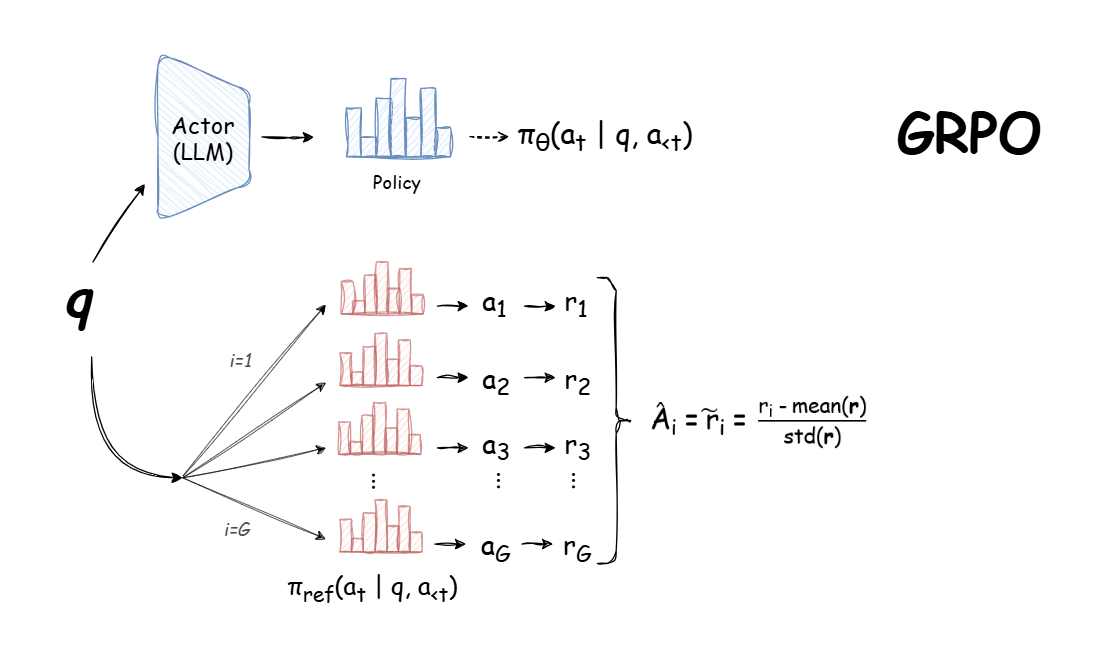
\includegraphics[width=0.82\textwidth]{images/GRPO}
  \caption{Vòng lặp huấn luyện GRPO. Từ mỗi prompt, policy sinh $G$
    completions; hàm reward chấm điểm từng completion; advantage được
    chuẩn hóa trong nhóm (group normalization); policy cập nhật với
    ràng buộc KL so với reference policy.}
  \label{fig:grpo-train}
\end{figure}

Advantage của completion $i$ trong nhóm $G$:

\begin{equation}
  A_i = \frac{r_i - \bar{r}}{\sigma_r + \varepsilon}, \quad
  \bar{r} = \frac{1}{G}\sum_{j=1}^{G} r_j, \quad
  \sigma_r = \sqrt{\frac{1}{G}\sum_{j=1}^{G}(r_j - \bar{r})^2}
  \label{eq:grpo-advantage}
\end{equation}

Hàm mất mát GRPO kết hợp ràng buộc KL so với reference policy
$\pi_{\text{ref}}$:

\begin{equation}
  \mathcal{L}_{\text{GRPO}}
    = -\frac{1}{G}\sum_{i=1}^{G} A_i \log \pi_\theta(y_i \mid x)
    + \beta \cdot D_{\text{KL}}\!\bigl(\pi_\theta \,\|\, \pi_{\text{ref}}\bigr)
  \label{eq:grpo-loss}
\end{equation}

với $\beta = 0{,}04$ là hệ số phạt KL ngăn policy lệch quá xa khỏi
mô hình nền ban đầu.

\subsection{Tập dữ liệu Dining Review}

Dữ liệu huấn luyện gồm 500 bài đăng thực thu thập từ cộng đồng
\emph{Dining Review} (Facebook) --- các bài viết review nhà hàng,
quán ăn tại Việt Nam bằng tiếng Việt. Mỗi bản ghi có 11 cột:
\texttt{text} (nội dung) và 10 chỉ số tương tác gồm
\texttt{likesCount}, \texttt{commentsCount}, \texttt{sharesCount},
và bảy loại reaction (like, love, haha, care, wow, angry, sad).

\textbf{Điểm engagement tổng hợp.} Từ các chỉ số tương tác, một
điểm proxy được xây dựng theo công thức trọng số:

\begin{equation}
  e_{\text{raw}} = L + 0{,}5C + 1{,}5S
    + R_{\text{like}} + 1{,}2\,R_{\text{love}}
    + 0{,}8\,(R_{\text{haha}} + R_{\text{care}} + R_{\text{wow}})
    - 0{,}5\,R_{\text{angry}} - 0{,}3\,R_{\text{sad}}
  \label{eq:engage-raw}
\end{equation}

\begin{equation}
  e = \ln\!\bigl(1 + \max(e_{\text{raw}},\, 0)\bigr)
  \label{eq:engage-log}
\end{equation}

trong đó $L$, $C$, $S$ lần lượt là lượt thích, bình luận, chia sẻ.
Trọng số cao hơn cho share ($1{,}5\times$) phản ánh cam kết sâu hơn;
hàm logarithm nén phân phối lệch phải của engagement. Tập train
dùng 256 mẫu, tập eval dùng 32 mẫu, lấy ngẫu nhiên từ 500 bài.

\textbf{Chiến lược Prefix Completion.} Dataset không có cặp
prompt--response rõ ràng. Giải pháp: câu đầu tiên của mỗi bài thực
đóng vai trò \emph{state/prompt}, phần còn lại do model sinh ra và
được hàm reward chấm điểm. Model học cách hoàn thiện bài post sao
cho các tín hiệu hình thức tương quan với engagement cao trong dataset.

\subsection{Hàm reward rule-based}

Hàm reward được thiết kế dựa trên phân tích tương quan giữa đặc trưng
hình thức và điểm engagement trong tập Dining Review. Năm thành phần
được mô tả trong Bảng~\ref{tab:reward-fn}.

\begin{table}[htbp]
  \centering
  \small
  \caption{Năm thành phần hàm reward rule-based và điểm số tương ứng.}
  \label{tab:reward-fn}
  \begin{tabular}{p{0.22\textwidth}cp{0.50\textwidth}}
    \toprule
    \textbf{Thành phần} & \textbf{Điểm} & \textbf{Điều kiện} \\
    \midrule
    \multirow{3}{*}{Độ dài}
      & $+1{,}0$ & $150 \leq |y| \leq 1\,000$ ký tự \\
      & $-2{,}0$ & $|y| < 30$ ký tự \\
      & $-0{,}5$ & $|y| > 2\,000$ ký tự \\
    \midrule
    Emoji
      & $+\min(0{,}15k,\; 0{,}6)$ & $k$: số emoji --- tương quan dương
        với likes và reactions trong dataset \\
    \midrule
    \multirow{2}{*}{CTA / câu hỏi}
      & $+0{,}4$ & Từ khoá gọi hành động (bình luận, chia sẻ, đặt bàn,
        inbox, liên hệ\ldots) \\
      & $+0{,}3$ & Có dấu hỏi (\texttt{?}) \\
    \midrule
    Kết thúc hoàn chỉnh
      & $+0{,}2$ & Ký tự cuối là dấu kết thúc
        (\texttt{.}, \texttt{!}, \texttt{?}, \texttt{…}) \\
    \midrule
    Tiếng Việt
      & $+0{,}3$ & $\geq 6$ ký tự có dấu --- đảm bảo model không
        sinh tiếng Anh \\
    \bottomrule
  \end{tabular}
\end{table}

\subsection{Cấu hình huấn luyện}

\texttt{Qwen3.5-2B} được chọn làm policy để giữ nhất quán với cấu
hình SFT, cho phép so sánh trực tiếp hiệu quả hai phương pháp trên
cùng mô hình nền. Bảng~\ref{tab:grpo-config} tóm tắt siêu tham số.

\begin{table}[htbp]
  \centering
  \small
  \caption{Siêu tham số huấn luyện GRPO.}
  \label{tab:grpo-config}
  \begin{tabular}{ll}
    \toprule
    \textbf{Tham số} & \textbf{Giá trị} \\
    \midrule
    Mô hình nền & \texttt{Qwen/Qwen3.5-2B} \\
    Quantization & QLoRA 16-bit (NF4, double quant, bf16 compute) \\
    LoRA & $r=16$, $\alpha=32$, dropout $=0$;
           7 module (q/k/v/o proj, gate/up/down proj) \\
    Tham số có thể huấn luyện & $10{,}9$M / $1{,}89$B ($0{,}58\%$) \\
    \midrule
    Số completions mỗi prompt ($G$) & 4 \\
    Độ dài completion tối đa & 256 token \\
    Nhiệt độ sinh ($T$) & $0{,}7$ \\
    Hệ số KL penalty ($\beta$) & $0{,}04$ \\
    \midrule
    Epochs & 1 \\
    Batch size / gradient accumulation & 1 / 4 (effective batch = 4) \\
    Learning rate & $3 \times 10^{-6}$ \\
    Số mẫu train / eval & 256 / 32 \\
    \bottomrule
  \end{tabular}
\end{table}

Kết quả đánh giá trên tập F\&B thực tế được trình bày cùng kết quả
SFT trong Bảng~\ref{tab:final-comparison}
(Mục~\ref{sec:tong-ket-thuc-nghiem}).

\section{Khung đánh giá chất lượng đa lớp}\label{sec:pipeline-danh-gia}

Để đánh giá chất lượng nội dung sinh ra một cách tự động hóa và có độ
tin cậy cao, luận văn xây dựng pipeline đánh giá ba lớp độc lập dựa
trên thư viện \textbf{DeepEval}. Mỗi lớp đo một chiều khác nhau của
chất lượng bài viết marketing; điểm tổng hợp kết hợp tuyến tính kết
quả từ cả ba lớp. Pipeline được hiện thực trong module
\texttt{evaluation/metrics.py} với kiến trúc thống nhất: mỗi
evaluator kết hợp một thành phần rule-based (nhanh, xác định) và một
thành phần LLM judge (ngữ nghĩa sâu hơn) qua lớp \texttt{JudgeLLM}
bọc OpenAI/AzureOpenAI client thành giao diện tương thích
\texttt{DeepEvalBaseLLM}.

\subsection{Lớp 1 --- Faithfulness: Kiểm tra tuân thủ thực thể}
\label{subsec:faithfulness}

Lớp này xác minh bài viết có trung thực với thông tin trong nội dung
mồi hay không, tránh hiện tượng \emph{hallucination} (bịa đặt giá,
tên sản phẩm, thông số). Điểm tổng hợp:

\begin{equation}
  \text{Faithfulness} = 0{,}5 \cdot s_{\text{rule}} + 0{,}5 \cdot s_{\text{llm}}
  \label{eq:faithfulness}
\end{equation}

\textbf{Thành phần quy tắc} ($s_{\text{rule}}$): lớp
\texttt{EntityPresenceRule} trích xuất năm nhóm thực thể từ seed
bằng biểu thức chính quy: giá tiền (VNĐ/đ/k/triệu/\%), thông số kỹ
thuật (ml/g/kg/kcal), combo/set/deal, chuỗi trích dẫn, và tên sản
phẩm/thương hiệu. Điểm là tỉ lệ thực thể xuất hiện trong đầu ra:

\begin{lstlisting}[language=Python, caption={EntityPresenceRule --- năm nhóm thực thể F\&B.}]
PRICE_RE = re.compile(
    r"(?:\d{1,3}(?:[.,]\d{3})+|\d+)\s*"
    r"(?:VND|dong|d|trieu|tr\.?|k)\b|[%$]",
    re.IGNORECASE)
SPEC_RE  = re.compile(
    r"\b\d+(?:[.,]\d+)?\s*(?:ml|lit|g|kg|kcal|cal)\b",
    re.IGNORECASE)
COMBO_RE = re.compile(
    r"\b(?:combo|set|deal|goi)\s*\d+|\d+\s*(?:mon|ly|to)\b",
    re.IGNORECASE)

def measure(self, seed, output):
    entities = self.extract_entities(seed)  # 5 loai tren
    if not entities:
        return 1.0, {"note": "no entities"}
    matched = [e for e in entities if e.lower() in output.lower()]
    return len(matched) / len(entities), {"matched": matched}
\end{lstlisting}

\textbf{Thành phần LLM} ($s_{\text{llm}}$): \texttt{FaithfulnessGEval}
(GEval của DeepEval) đánh giá mâu thuẫn giữa đầu ra và retrieval
context bằng chain-of-thought, trừ điểm nếu output chứa claim không
được hỗ trợ bởi seed (kể cả hype vô căn cứ).

\subsection{Lớp 2 --- Expansion Quality: Đánh giá khả năng mở rộng}
\label{subsec:expansion}

Lớp này đo lường khả năng mô hình \emph{diễn giải} thông tin kỹ thuật
thô thành nội dung có giá trị với khách hàng, thay vì chỉ liệt kê lại.
Điểm tổng hợp:

\begin{equation}
  \text{Expansion} = 0{,}9 \cdot s_{\text{llm}} + 0{,}1 \cdot s_{\text{rule}}
  \label{eq:expansion}
\end{equation}

\textbf{Thành phần LLM} ($s_{\text{llm}}$): \texttt{ExpansionGEval}
với tiêu chí: ``Bài phải diễn giải lợi ích cho khách hàng và ngữ cảnh
sử dụng thực tế từ thông tin thô trong seed. Trừ điểm nếu chỉ lặp lại
bullet kỹ thuật mà không giải thích giá trị.''

\textbf{Thành phần quy tắc} ($s_{\text{rule}}$):
\texttt{ContentExpansionRule} đo ba tín hiệu:
(i)~\emph{tỉ lệ độ dài} $s_{\text{len}}$ ($r \geq 2{,}5 \to 1{,}0$;
$r \geq 1{,}5 \to 0{,}7$; $r \geq 1{,}0 \to 0{,}4$; còn lại $0{,}1$);
(ii)~\emph{ngôn ngữ lợi ích} $s_{\text{ben}} = \min(1, n_{\text{ben}}/3)$
(từ khóa ``giúp'', ``tận hưởng'', ``phù hợp'',...);
(iii)~\emph{ngữ cảnh sử dụng} $s_{\text{ctx}} = \min(1, n_{\text{ctx}}/2)$
(từ khóa dịp/thời điểm). Kết hợp:
$s_{\text{rule}} = 0{,}4\,s_{\text{len}} + 0{,}35\,s_{\text{ben}} +
0{,}25\,s_{\text{ctx}}$.

\subsection{Lớp 3 --- Marketing Vibe: Đánh giá phong cách marketing}
\label{subsec:vibe}

Lớp này đánh giá chất lượng phong cách theo tiêu chuẩn
Facebook-native F\&B tiếng Việt, kết hợp LLM judge 5 chiều,
cấu trúc Facebook và điểm phạt:

\begin{equation}
  \text{Vibe} = \max\!\Bigl(0,\,\min\!\Bigl(1,\;
  0{,}85\,s_{\text{llm}} + 0{,}15\,s_{\text{fb}} - p\Bigr)\Bigr)
  \label{eq:vibe}
\end{equation}

\textbf{LLM judge 5 chiều} ($s_{\text{llm}}$):
\texttt{MarketingVibeJudge} gửi rubric đặc thù cho judge LLM, nhận
điểm nguyên $0$--$4$ trên từng chiều D1--D5, rồi tính:
$s_{\text{llm}} = \sum_k w_k \cdot d_k / 4$.

\begin{table}[h]
  \centering
  \small
  \caption{Năm chiều đánh giá Vibe và trọng số.}
  \label{tab:vibe-dims}
  \begin{tabular}{cp{0.65\textwidth}c}
    \toprule
    \textbf{Chiều} & \textbf{Mô tả} & \textbf{Trọng số} \\
    \midrule
    D1 & Giọng thật --- trực tiếp, không brand-speak/AI template & 0,25 \\
    D2 & Neo thực tế kinh doanh --- giá, deal, combo, thời hạn & 0,15 \\
    D3 & Thuyết phục bằng cụ thể --- số liệu, không hype rỗng & 0,25 \\
    D4 & Chất lượng CTA --- token hành động rõ, low-friction & 0,20 \\
    D5 & Nhịp Facebook tự nhiên --- đoạn ngắn, không AI essay & 0,15 \\
    \bottomrule
  \end{tabular}
\end{table}

\textbf{Cấu trúc Facebook} ($s_{\text{fb}}$):
\texttt{FbStructureRule} đo bốn tín hiệu có trọng số: tỉ lệ đoạn
ngắn ($\leq 320$ ký tự), độ dài đoạn trung bình ($\leq 280$ ký tự),
có danh sách gạch đầu dòng, và có dòng CTA tường minh.

\textbf{Điểm phạt} ($p$): \texttt{VibePenaltyRule} trừ điểm cho bốn
lỗi phong cách: ngôn ngữ phóng đại ($-0{,}10$), câu mở kiểu AI
($-0{,}08$), emoji quá dày ($-0{,}05$), và bullet list rập khuôn
($-0{,}05$).

\subsection{Điểm tổng thể và ngưỡng phê duyệt}

Điểm tổng thể là trung bình cộng của ba lớp:

\begin{equation}
  \text{Overall} = \frac{1}{3}(\text{Faithfulness} + \text{Expansion} + \text{Vibe})
  \label{eq:overall}
\end{equation}

Trong triển khai, bài đạt $\text{Overall} \geq \theta = 0{,}75$ được
chuyển tự động sang trạng thái \texttt{approved}. Ngưỡng $\theta$ có
thể cấu hình theo từng dự án mà không cần thay đổi code pipeline.

\section{Tổng kết kết quả thực nghiệm fine-tuning}
\label{sec:tong-ket-thuc-nghiem}

Bảng~\ref{tab:final-comparison} tổng hợp toàn bộ kết quả trên tập
F\&B thực tế ($n = 100$, judge: GPT-5.4 Azure) cho ba hướng tiếp cận:
mô hình nền chưa tinh chỉnh, SFT (Supervised Fine-Tuning), và GRPO
(học tăng cường với reward rule-based). Tất cả mô hình mã nguồn mở
sinh văn bản ở chế độ \emph{nothinking}, nhiệt độ $T = 0{,}4$; GPT-5.4-mini
là điểm tham chiếu thương mại.

\begin{table}[htbp]
  \centering
  \small
  \caption{So sánh tổng hợp mô hình nền, SFT và GRPO trên tập F\&B
    thực tế ($n=100$, judge: GPT-5.4 Azure). In đậm: cao nhất mỗi cột
    trong nhóm mã nguồn mở.}
  \label{tab:final-comparison}
  \begin{tabular}{lcccc}
    \toprule
    \textbf{Mô hình} & \textbf{Faith.} & \textbf{Expan.}
      & \textbf{Vibe} & \textbf{Overall} \\
    \midrule
    GPT-5.4-mini (baseline thương mại)
      & 0,659 & 0,817 & 0,645 & 0,707 \\
    \midrule
    \texttt{qwen3.5:2b} (nền)
      & 0,599 & 0,662 & 0,450 & 0,570 \\
    \texttt{qwen3.5:2b} + SFT
      & 0,597 & 0,754 & 0,587 & 0,646 \\
    \texttt{qwen3.5:2b} + GRPO
      & \multicolumn{4}{c}{\textit{đang đánh giá}} \\
    \midrule
    \texttt{qwen3.5:4b} (nền)
      & 0,596 & 0,768 & 0,502 & 0,622 \\
    \texttt{qwen3.5:4b} + SFT
      & \textbf{0,637} & \textbf{0,777} & \textbf{0,648} & \textbf{0,687} \\
    \midrule
    \texttt{qwen3.5:9b} (nền, tham chiếu)
      & 0,584 & 0,780 & 0,538 & 0,634 \\
    \bottomrule
  \end{tabular}
\end{table}

\textbf{SFT cải thiện Vibe rõ rệt ở cả hai kích thước.}
\texttt{qwen3.5:2b} + SFT tăng Vibe từ 0,450 lên 0,587 ($+30{,}4\%$);
\texttt{qwen3.5:4b} + SFT từ 0,502 lên 0,648 ($+29{,}1\%$). Đây là
lớp hưởng lợi nhiều nhất từ tinh chỉnh có giám sát, xác nhận rằng
giọng điệu Facebook-native F\&B có thể học được từ dữ liệu kiểm duyệt.

\textbf{Expansion cải thiện rõ trên 2B, ổn định trên 4B.}
\texttt{qwen3.5:2b} + SFT tăng từ 0,662 lên 0,754 ($+0{,}092$), trong
khi \texttt{qwen3.5:4b} + SFT giữ nguyên (0,768 $\to$ 0,777) vì mô
hình 4B đã có năng lực diễn giải nội sinh từ tiền huấn luyện.

\textbf{Faithfulness ổn định qua fine-tuning.} Cả hai mô hình SFT
không giảm Faithfulness đáng kể (2B: $-0{,}002$; 4B: $+0{,}041$),
xác nhận SFT không làm mất khả năng bảo toàn thực thể --- điều kiện
cần cho triển khai thực tế.

\textbf{GRPO bổ sung tín hiệu tương tác thực.} Khác với SFT học từ
nhãn kiểm duyệt, GRPO tối ưu trực tiếp theo các đặc trưng hình thức
tương quan với engagement trong tập Dining Review (500 bài). Hai
hướng tiếp cận có thể kết hợp tuần tự --- SFT định hình phong cách
từ bài mẫu đã duyệt, GRPO tinh chỉnh tiếp theo phản hồi tương tác
thực --- tạo thành pipeline huấn luyện đa giai đoạn phù hợp với SME.

\textbf{\texttt{qwen3.5:4b} + SFT là lựa chọn tốt nhất trong nhóm
mã nguồn mở hiện tại}, với Overall 0,687 so với 0,707 của GPT-5.4-mini
($\Delta = -0{,}020$, $-2{,}8\%$). Chi phí vận hành thấp hơn đáng kể
(mô hình cục bộ, không phụ thuộc API thương mại theo lượt gọi) mang
lại ý nghĩa thực tiễn cho SME ngành F\&B Việt Nam.
